\documentclass[aspectratio=169]{beamer}
\usepackage{tikz}
\usepackage{graphicx}
\usepackage{listings}
\usepackage{xcolor}
\usepackage{hyperref}
\usepackage[spanish,es-noquoting]{babel}
\usepackage[round]{natbib}

\lstset{
  basicstyle=\ttfamily\small,
  keywordstyle=\color{blue},
  stringstyle=\color{red},
  commentstyle=\color{gray},
  showstringspaces=false
}
% Minimal look
\usetheme{Warsaw}
%\setbeamertemplate{headline}
\setbeamertemplate{footline}{
  \leavevmode%
  \hbox{%
    % Left: Section name
    \begin{beamercolorbox}[wd=.33\paperwidth,ht=2.25ex,dp=1ex,left]{author in head/foot}%
      \hspace*{2ex}\insertsection
    \end{beamercolorbox}%
    % Center: Presentation title
    \begin{beamercolorbox}[wd=.34\paperwidth,ht=2.25ex,dp=1ex,center]{title in head/foot}%
      \insertshorttitle
    \end{beamercolorbox}%
    % Right: Slide numbers
    \begin{beamercolorbox}[wd=.33\paperwidth,ht=2.25ex,dp=1ex,right]{date in head/foot}%
      \insertframenumber{} / \inserttotalframenumber\hspace*{2ex}
    \end{beamercolorbox}%
  }%
  \vskip0pt%
}

\usecolortheme{default}
\usefonttheme{serif}
\graphicspath{{../}{./}}
\setbeamertemplate{caption}[numbered]

% Title info
\title[ Transformación de la Práctica]{ Transformación de la Práctica Jurídica}
\subtitle{ Lo que la IA sí puede (y no puede) hacer}
\author{Ricardo Reyes-Jimenez}
\institute{Universidad de La Sabana}
\date{\today}

% Background image for title slide
\usebackgroundtemplate{
  \tikz\node[opacity=0.3]{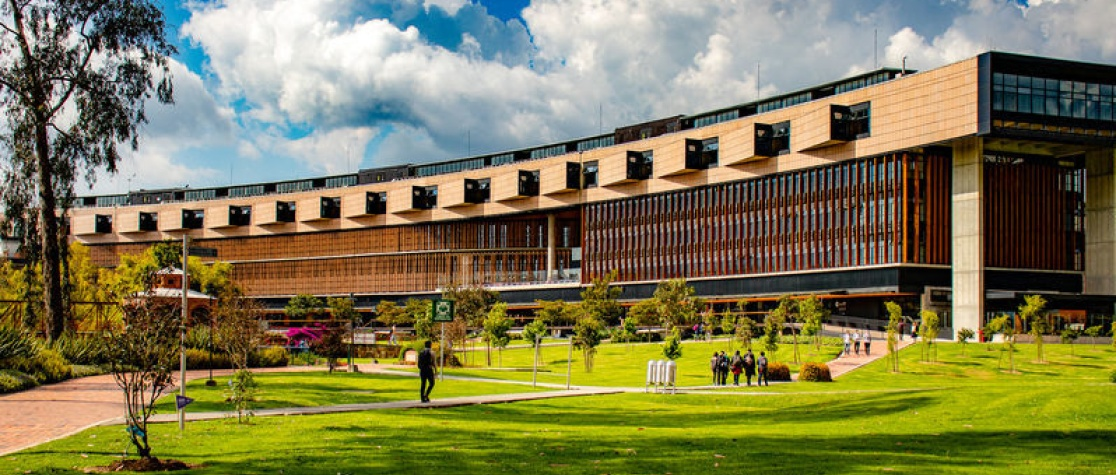
\includegraphics[width=\paperwidth,height=\paperheight]{Images/UniSabana.jpg}};
}

\begin{document}

% Title slide
\begin{frame}
  \titlepage
\end{frame}

% Reset background for normal slides
\usebackgroundtemplate{}



\begin{frame}[fragile]{Introducción al Módulo 1.2}


Este módulo profundiza en cómo la Inteligencia Artificial Generativa está cambiando la práctica jurídica diaria, estableciendo qué tareas pueden delegarse de manera segura y cuáles son los límites técnicos actuales.

\end{frame}



\begin{frame}[fragile]{Ética y Uso Responsable (Gemini)}


El análisis de documentos legales con IA exige un estándar ético riguroso:

\begin{itemize}
  \item \textbf{Privilegio Abogado-Cliente:} El abogado sigue siendo el garante del secreto profesional.
  \item \textbf{Sesgos y Equidad:} La IA puede heredar sesgos de sus datos de entrenamiento.
  \item \textbf{Responsabilidad de Uso (Gemini):} Se debe usar como asistente y no como tomador de decisiones. El output debe ser siempre revisado por un humano.
\end{itemize}
\end{frame}



\begin{frame}[fragile]{Creación de Prompts Estructurados}


¿Por qué usar formatos estructurados en vez de texto plano?

El texto plano requiere lectura humana para interpretar dónde empieza y termina un dato. Los formatos estructurados permiten que otras herramientas informáticas extraigan la información automáticamente sin errores.

\begin{itemize}
  \item \textbf{JSON (JavaScript Object Notation):} Formato universal basado en ``llave: valor''. Ideal para extraer metadatos puros (ej. `{``vencimiento'': ``2024-12-31''}`).
  \item \textbf{.MD (Markdown):} Formato de texto con marcas ligeras (como `\#` para títulos o `*` para listas). Ideal para generar borradores de documentos legales o memos que mantengan formato de lectura fácil.
\end{itemize}
\textbf{Ejemplo:} \textit{``Extrae las fechas de vencimiento y preséntalas en un JSON estructurado por partes involucradas.''}

\end{frame}



\begin{frame}[fragile]{Ejemplo de Salida: JSON vs .MD}


\begin{columns}[T]
\begin{column}{0.48\textwidth}
\textbf{Salida en JSON}
\begin{lstlisting}[basicstyle=\ttfamily\scriptsize]
{
``contrato'': {
``tipo'': ``[Ej: Arrendamiento]'',
``partes'': [
``[Nombre Parte 1]'',
``[Nombre Parte 2]''
],
``vencimiento'': ``YYYY-MM-DD'',
``penalidad'': ``[Resumen]''
}
}
\end{lstlisting}
\end{column}

\begin{column}{0.48\textwidth}
\textbf{Salida en Markdown}
\begin{lstlisting}[basicstyle=\ttfamily\scriptsize]
### Datos del Contrato
\begin{itemize}
  \item \textbf{Tipo:} [Ej: Arrendamiento]
\end{itemize}
### Partes Involucradas
1. [Nombre Parte 1]
2. [Nombre Parte 2]

### Fechas y Condiciones
\begin{itemize}
  \item \textbf{Vencimiento:} YYYY-MM-DD
  \item \textbf{Penalidad:} [Resumen]
\end{itemize}
\end{lstlisting}
\end{column}
\end{columns}

\end{frame}



\begin{frame}[fragile]{Privacidad: ¿A dónde va la información?}


El uso de modelos gratuitos (como ChatGPT o Gemini básico) conlleva riesgos de privacidad:

\begin{itemize}
  \item \textbf{Modelos Gratuitos:} Por defecto, los datos ingresados (prompts) \textbf{pueden ser utilizados} para entrenar futuras versiones del modelo \cite{geminiprivacy}.
  \item \textbf{Pérdida de Confidencialidad:} Introducir datos reales de un cliente en estas versiones viola los deberes éticos.
  \item \textbf{Solución:} Utilizar versiones \textbf{Enterprise/Corporativas}, modelos locales, o desactivar explícitamente el uso de datos para entrenamiento.
\end{itemize}
\end{frame}



\begin{frame}[fragile]{Recapitulemos}


\begin{figure}\centering
\includegraphics[height=0.6\textheight,keepaspectratio]{Images/Slido1.png}\caption{¿Cómo te sientes?}\end{figure}

\href{https://app.sli.do/event/225ytceXVMF9WqQb2yXQcp}{https://app.sli.do/event/225ytceXVMF9WqQb2yXQcp}

\end{frame}



\begin{frame}[fragile]{Lo que la IA SÍ puede (y NO puede) hacer}


\begin{table}
\resizebox{\textwidth}{!}{
\begin{tabular}{|l | l | l|}
\hline
\textbf{Tarea Jurídica} & \textbf{Nivel de Riesgo} & \textbf{Recomendación} \\ \hline
Redacción de correos y memos simples & Bajo & Uso rutinario con supervisión básica \\ \hline
Búsqueda de jurisprudencia en bases abiertas & Alto & NO RECOMENDADO (Riesgo de alucinación) \\ \hline
Resumen de expedientes largos & Medio & Ideal para IA, validando contra el PDF original \\ \hline
Análisis predictivo de sentencias & Alto & Requiere herramientas especializadas (ej. Lexis+ AI) \\ \hline
\end{tabular}
}
\end{table}
\end{frame}



\begin{frame}[fragile]{Sondeo}


\begin{figure}\centering
\includegraphics[height=0.6\textheight,keepaspectratio]{Images/Slido2.png}\caption{Usos posibles}\end{figure}

\href{https://app.sli.do/event/d4t1CEhzQVnvahXucVLCqT}{https://app.sli.do/event/d4t1CEhzQVnvahXucVLCqT}

\end{frame}



\begin{frame}[fragile]{Casos de Uso Reales en la Práctica}


\begin{itemize}
  \item \textbf{Investigación y Análisis Legal:} Utilizar la IA para encontrar patrones en grandes volúmenes de documentos, no para buscar la ``verdad'' legal.
  \item \textbf{Revisión de Contratos:} Identificar cláusulas faltantes o riesgosas (Ej. cláusulas de indemnidad asimétricas).
  \item \textbf{Orientación a Clientes:} Redactar respuestas iniciales en lenguaje claro y accesible.
  \item \textbf{Gestión Documental:} Extracción de metadatos (fechas, partes, montos) de expedientes masivos.
\end{itemize}
\end{frame}



\begin{frame}[fragile]{El Peligro de la Confianza Ciega (Mata v. Avianca)}


\textbf{El puente entre el potencial y el riesgo:}

En 2023, abogados en EE. UU. usaron ChatGPT para investigar jurisprudencia y presentaron un escrito con casos que la IA \textbf{inventó (alucinó)} \cite{matavavianca}.

\begin{itemize}
  \item Fueron sancionados por el juez.
  \item Demostró que delegar la investigación sin verificación es negligencia profesional grave.
\end{itemize}
\end{frame}



\begin{frame}[fragile]{Límites Críticos de la IA Generativa}


\begin{itemize}
  \item \textbf{Falta de Actualización:} Los modelos fundacionales tienen una fecha de corte de conocimiento. No conocen la ley aprobada ayer.
  \item \textbf{Falta de Hechos Específicos:} La IA no conoce el contexto único de su cliente a menos que usted se lo proporcione.
  \item \textbf{Alucinaciones:} La tendencia de la IA a inventar respuestas plausibles pero falsas cuando no tiene información suficiente.
\end{itemize}
\end{frame}



\begin{frame}[fragile]{Protocolo de Verificación Legal}


\begin{itemize}
  \item \textbf{Grounding (Anclaje):} Proporcionar a la IA los documentos fuente sobre los cuales debe basar su respuesta.
  \item \textbf{Prompts Restrictivos:} Instruir explícitamente a la IA: ``Responde ÚNICAMENTE basado en los documentos adjuntos''.
  \item \textbf{Verificación Humana:} El abogado siempre debe revisar el documento final. La responsabilidad legal recae en el humano.
\end{itemize}
\end{frame}



\begin{frame}[fragile]{Flujo de Verificación (Ejemplo Práctico)}


\begin{center}
\resizebox{0.9\textwidth}{!}{
\begin{tikzpicture}[node distance=3cm, auto, thick,
box/.style={rectangle, draw=blue!80, fill=blue!10, very thick, text width=3.5cm, align=center, rounded corners, minimum height=1.5cm},
arrow/.style={->, >=stealth, very thick, blue!80}]
\node[box] (n1) {1. Subir PDF del Contrato (Grounding)};
\node[box, right of=n1, xshift=1.5cm] (n2) {2. Prompt restrictivo con formato JSON};
\node[box, right of=n2, xshift=1.5cm] (n3) {3. Verificar JSON contra original};
\draw[arrow] (n1) -- (n2);
\draw[arrow] (n2) -- (n3);
\end{tikzpicture}
}
\end{center}

\end{frame}



\begin{frame}[fragile]{Tu Opinión}


\begin{figure}\centering
\includegraphics[height=0.6\textheight,keepaspectratio]{Images/Slido3.png}\caption{Ética y Responsabilidad}\end{figure}

\href{https://app.sli.do/event/9jutLvGy9zr5HcmKtmq1nd}{https://app.sli.do/event/9jutLvGy9zr5HcmKtmq1nd}

\end{frame}



\begin{frame}[fragile]{Ejercicio Práctico: Grounding con NotebookLM}


\textbf{Herramienta:} Gemini Notebook \cite{notebooklm2024}

\textbf{Objetivo:} Interactuar con un expediente masivo sin riesgo de alucinaciones.

\begin{itemize}
  \item Subir la sentencia o expediente en PDF.
  \item Generar una guía de estudio automática.
  \item Hacer preguntas específicas al documento.
  \item Verificar las citas (Gemini Notebook muestra de qué página extrajo la información).
\end{itemize}
\end{frame}



\begin{frame}[allowframebreaks]{Referencias}
  \bibliographystyle{apalike}
  \bibliography{references}
\end{frame}

\begin{frame}[fragile]{¡Sigamos en Contacto!}


La Inteligencia Artificial avanza todos los días. ¡No duden en escribirme para compartir ideas, resolver dudas o seguir conversando sobre cómo la IA puede transformar su práctica jurídica!

\begin{itemize}
  \item \textbf{WhatsApp:} (57) 3012726157
  \item \textbf{Email:} \href{mailto:rareyesj@gmail.com}{rareyesj@gmail.com}
\end{itemize}
\textbf{¡Muchas gracias por su participación!}
\end{frame}





\end{document}